\chapter{为回顾做好准备} % Introduction chapter suppressed from the table of contents

\framebox{%
\begin{minipage}[t]{0.97\columnwidth}\raggedright
\textbf{请你按过去一年的软件开发项目,按工种占项目总工作量,从最多排到最少?}

\begin{enumerate}
\tightlist
\item
  设计与编码
\item
  交付后的所有工作,包括维护、更新与缺陷修正
\item
  交付前的评审,静态扫描,测试与缺陷修正
\item
  项目管理与监控
\end{enumerate}\strut
\end{minipage}}

可看附件中的``开发项目工作量(成本)分布'',看你的选择与`典型'分布差多远。

软件开发项目通常最大的成本是花在找出与修正缺陷。

按专家Capers JONES 先生2012年的研究,
超过10,000功能点,计划能使用25年的大型系统,接近一半的工作量都是与找出与修正缺陷相关。

\begin{description}
\item[]
\begin{description}
\tightlist
\item[]
= = =
\end{description}
\end{description}

初次见软件研发总监,我会问:``通常你们的项目在哪个过程中发现的缺陷最多?''

\begin{description}
\item[]
\begin{description}
\tightlist
\item[]
超过95\% 都会说最多是在系统测试,或验收测试阶段发现\\
\end{description}
\end{description}

%\url{文件:AR1缺陷数.jpg}

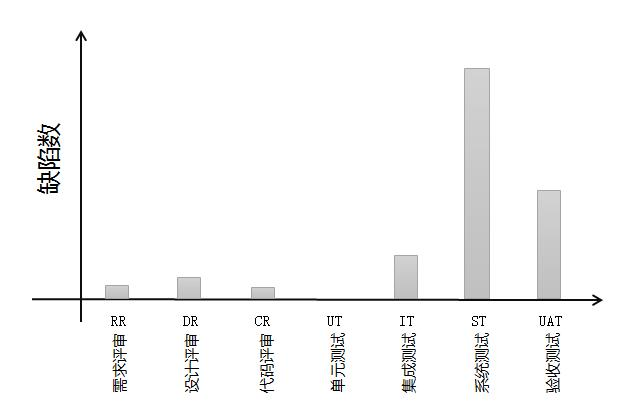
\includegraphics[width=10cm]{AR1缺陷数.jpg}

再问:用于测试与缺陷修复的返工的总工作量占整个开发项目多少?

大部分领导都没有概念。

我总结:如果能把后面发现的缺陷,提前在前面预先发现,估计可以节省多少工作量?

\framebox{%
\begin{minipage}[t]{0.97\columnwidth}\raggedright
当我在白板上估算出,如果能把系统测试发现的缺陷数减半,总的工作量会减少,研发成本也会降低,很多总监都会觉得不可思议,因他们一直都已经习惯了后面测试缺陷多,觉得是常态。\strut
\end{minipage}}

\hypertarget{ux7f3aux9677ux6392ux9664ux7387-dre}{%
\subsection{缺陷排除率 (DRE)}\label{ux7f3aux9677ux6392ux9664ux7387-dre}}

%\href{文件:jalote_emm_7.1_1.0.png}{500px}

\includegraphics[width=10cm]{jaloteemm7110.png}

Figure7.1,从需求到设计、编码、单元测试、系统测试、验收,整个开发过程大家都很熟悉(缺陷只会源自需求、设计、编码);需求、设计、编码后都会评审/测试来排除缺陷,但仅仅做评审/测试不一定能确保质量。因为最终验收缺陷数取决于每个步骤能否有效排除当前的缺陷。

所以可以用缺陷排除率(Defect Removal Efficiency DRE)
来衡量测试或评审的效率:

%\href{文件:Ma3_1.0.png}{文件:Ma3 1.0.png}

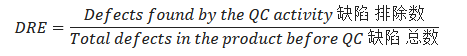
\includegraphics[width=10cm]{Ma310.png}

缺陷排除率除了可以用于整个项目,包括测试,也可以用于前面评审、扫描等。

\begin{description}
\item[]
\begin{description}
\tightlist
\item[]
= = =
\end{description}
\end{description}

有些人会认为尽早发现并解决缺陷
对质量肯定好,但会耗费工作量,增加项目成本,老板不一定愿意。
其实是反过来,如能在前面预先发现并修正缺陷,
便能减小后面测试和修改缺陷的工作量, 最终只会减少总项目工作量。

%\href{文件:AR1FixVarCostScreenshot_2022-12-10_144400.jpg}{600px}

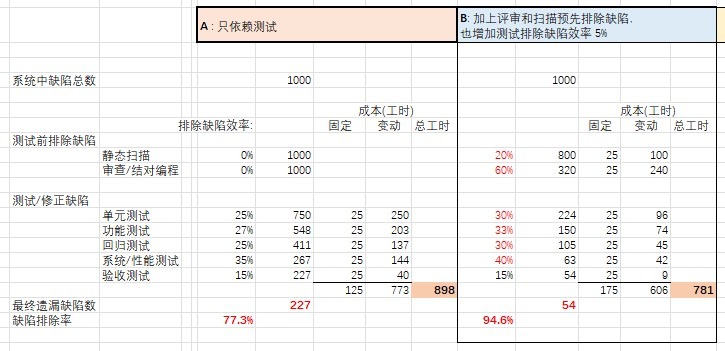
\includegraphics[width=10cm]{AR1FixVarCostScreenshot20221210144400.jpg}

比较以上两种策略的质量成本(COQ)就能看出:

\begin{itemize}
\tightlist
\item
  增加测试前扫描与审查,并加大测试效率,不仅减少最终缺陷数到54(对比227),也降低总质量成本(总人时)
\end{itemize}

%Screenshotfrom20221221203231.png

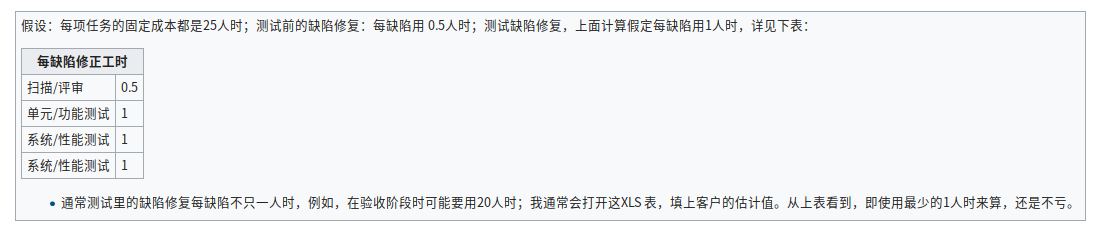
\includegraphics[width=10cm]{Screenshotfrom20221221203231.png}



因为缺陷已经提前被排除系统测试的缺陷减少,测试阶段的工作量减少大于前面扫描评审上的投入。

可以进一步利用COQ概念,增加早期预防缺陷措施,如用原型与客户交流,做好需求调研,进一步减少缺陷,和成本。
例如,使用原型与场景与客户挖掘需求,可进一步把缺陷降到43,也降低总质量成本:

%\href{文件:est缺陷表3.jpg}{600px}

\includegraphics[width=10cm]{est缺陷表3.jpg}

\texttt{注:你可能会质疑使用原型方法不只25人时,但即使加大到100人时,还是不亏。因它能预防缺陷,整体缺陷数下降20\%,使总质量成本下降超过100人时。}

正如质量大师Dr JURAN 强调,过程改进必须从认同必须改善质量(Proof of the
Need)开始。如果大家都觉得现在的缺陷水平(例如,系统测试超过200个缺陷)是常态,任何公司级质量改进计划都不会有好结果。\\
但如果管理层了解现在未能尽早发现并排除缺陷是最好的改进方向(80/20原则),并开始重视,但应如何开始?\\
``如何能收集到修复缺陷相关工时数据?因没有度量,便无法谈改进。我们现在只有缺陷数据,与测试工作量数据。''\\
收集软件开发数据不容易,但如果没有收集到可信的数据,便无从分析与改进。\\
是否可以靠组织级加强这方面相关的度量与监控?我们先看看一家几千人的大公司,他们一直都很强调量化管理,收集各种项目的系数,度量并分析。\\

\hypertarget{ux81eaux52a8ux5316ux7edfux8ba1ux5206ux6790}{%
\subsection{自动化统计分析}\label{ux81eaux52a8ux5316ux7edfux8ba1ux5206ux6790}}

客户:我们每次都跑全量,公司引入低码平台,更多的是在需求设计阶段做好质量保证,
所以我们很注重量化质量管理,能否通过自动化来统计分析?
如何通过量化或工具方式实现自动评审?

我:为什么要自动化?

客户:从去年开始我们搞度量分析, 发现员工就会造数据, 结果导致失真,
度量哪里就造哪里,
所以还是想通过工具代替人工方式,除了能提升效率,也能帮助判断数据是否合理。\\
现在我们的主管很反感度量,一度量就有人造数据

我:度量本来是件好事

客户:是的,就是大家知道算法原理就开始造假。 因为我们搞了红黑榜,
但很多人头脑都很聪明,会想办法,但用于不合适的地方。

我们有很多数据统计分析,比如看测试用例与需求的比例。
其实客户发现的缺陷比例也降低了,但因为我们这行对质量特别注重,产品经过多年的逐步演化,过程很复杂,导致软件缺陷的修复很耗时,客户不太满意。
而且公司要求交付的频率要比以前高了很多,我们团队做这些分析都忙不过来,所以需要员工设自动化工具等加快速度才可以。\\
让我给你看看我们大数据分析。。。

我:等等,但我们首要解决如何能收集到真正的数据,不然数据分析没有意义。

客户:好的,有什么建议?

我:还记得我们上次交流,要让团队自主,不能单靠标准过程并用指标监控执行情况?

%\href{文件:Diagram_2.0.png}{500px}

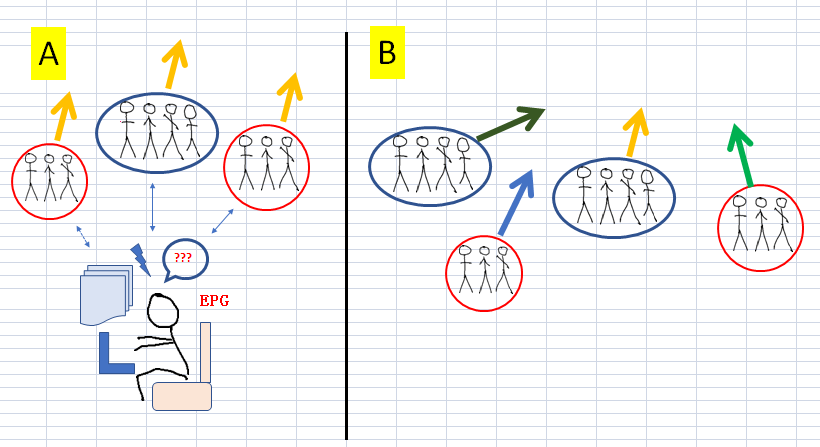
\includegraphics[width=10cm]{Diagram20.png}

我:请问你们是采用左面还是右面的方法做过程改进?\\
客户:好像我们现在度量分析是采用你图里左面的方法。

我:是的。总体分析还有另一不足:各个项目特性不一样,你们现在几十个项目总体趋势分析,
很可能找不对根因,因每个项目的问题(根本原因)很可能不同。
比如,同样是一个测试用例比例数,你的范围就很宽 -
从最低的0.3到最高的超过200!但你们取平均值5.1 来做分析。

收集数据也是问题,因收集数据是挺花精力的工作

客户:完全同意

我:但正因为不同项目有各种特性,要对收集到的数据做分析也很耗时。
这些辛辛苦苦做出来的分析报告其实不仅仅是给高层(或者项目经理),
在每一个团队成员都看到才有意义
。(度量分析要反馈回数据提供者,他们才有动力继续收集数据)要把那些分析好的报告再跟每一个团队成员解释上要花多大精力?

\textbf{度量的主要目的是从数据分析找出根因做改进而不是仅仅为了监控}

%\href{文件:Ma4CarScreenshot_2021-12-27_205004.png}{400px}

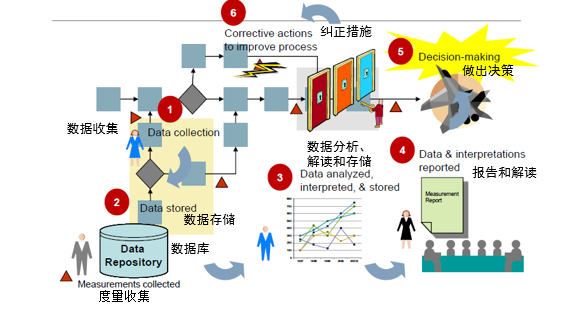
\includegraphics[width=10cm]{Ma4CarScreenshot20211227205004.png}

如果把数据分析下放到团队自己搞,便灵活多了;也正因为他们有参与收集和分析讨论,
你们也可以节省很多沟通的成本。

所以你们领导应该定位自己是内部老师,辅导团队怎么做好数据分析,效果会更好。

客户:就当团队自己讨论便可以得到改进吗?不需要我们领导?\\
我:
如果团队有能力,应该放手让他们自己利用收集数据,分析做改进。你们管理者应从以前分析数据,定位为团队的教练,辅导他们。千万不要误以为比以前自己做分析轻松,你们须要更熟悉,但因你们之前有经验,所以辅导团队应不会太难。更大的挑战反而是要管理层了解并赞同敏捷开发的团队自主思路。

\framebox{%
\begin{minipage}[t]{0.97\columnwidth}\raggedright
从Brehm 1956实验(详见附件)看到:

\begin{itemize}
\tightlist
\item
  我们都会对自己的选择更满意
\end{itemize}

从二战实验(详见附件)看到:

\begin{itemize}
\tightlist
\item
  我们只会执行自己讨论出来的选择(但不会遵循其他人,例如专家的建议)
\end{itemize}

所以要让团队自己收集数据,自己分析数据并讨论出改进方案,他们才有动力去执行。\strut
\end{minipage}}

\hypertarget{ux603bux7ed3}{%
\subsubsection{总结}\label{ux603bux7ed3}}

从以上的对话可以了解到,要量化管理不能单靠从上而下推,而必须让团队参与,团队才会提升,公司才会提升。假如团队成员按照前面PSP的思路,统计自己工作量、缺陷等,敏捷团队就可以在迭代回顾(或复盘)时,分析过去迭代的数据,并找出根本原因,在下一个迭代做对应纠正措施。\\
要让团队自己收集数据,分析数据,他们才有动力持续改进。
但团队首先要知道收集数据后如何分析,下章会分享关于根本原因分析的原理、方法与案例。

\hypertarget{ux9644ux4ef6}{%
\section{附件}\label{ux9644ux4ef6}}

\hypertarget{ux8d28ux91cfux6210ux672c-coq-cost-of-quality}{%
\subsection{质量成本 COQ (Cost of
Quality)}\label{ux8d28ux91cfux6210ux672c-coq-cost-of-quality}}

质量成本由三部分组成:

\begin{enumerate}
\tightlist
\item
  失效(Failure)成本\\
  把缺陷修复好的成本,包括在客户现场被发现的缺陷。
\item
  评测(Appraisal)成本\\
  包括各类测试,如系统测试,集成测试,单元测试等,所花的工时
\item
  预防(Prevention)成本\\
  包括技术评审 (注:有些人把评审归为评测成本,这里按 Mr.Juran
  定义,归属于预防成本)
\end{enumerate}

如变通理解以上COQ定义,``如何通过提高评审效率来降低质量成本``便可对应COQ各部分:\\
失效(Failure)成本:原本所有与缺陷相关的成本\\
评测(Appraisal)成本:增加测试前的静态扫描、评审,减少失效(Failure)成本,使总COQ下降\\
预防(Prevention)成本:减小缺陷的产生,例如用原型做好需求,进一步使总COQ下降\\

\hypertarget{brehm-1956-ux51b3ux7b56ux5f71ux54cdux5b9eux9a8c}{%
\subsection{Brehm 1956
决策影响实验}\label{brehm-1956-ux51b3ux7b56ux5f71ux54cdux5b9eux9a8c}}

\textbf{实验设计}:

\begin{enumerate}
\tightlist
\item
  提供十多种不同礼物,包括台灯,多士炉,挂钟、收音机、等
\item
  请你按自己喜好对礼物排序
  。例如,最喜欢的选一,如果同样喜欢两件礼物,可以不分高低,写同一个数字
\item
  让你从两件同样喜好的礼物,让你选其中一件,让你拿走
\item
  但在你离开之前,请你再对所有礼物按喜好排序
\end{enumerate}

\textbf{结果}:

\begin{itemize}
\tightlist
\item
  绝大部分人都会抬高自己选择拿走的那一件礼物排序,调低非选择的那件礼物排序
\item
  但如果不是自己选择,而是由老师选好给你,你后面的礼物排序就没有变化
\end{itemize}

\textbf{结论}:

\begin{itemize}
\tightlist
\item
  人都会觉得自己的选择比较好
\item
  例如,选大学,选汽车,选伴侣;如果是由你自己决定选择(非被安排),你会不会都会觉得自己的选择较好
\end{itemize}

\hypertarget{ux7caeux98dfux5206ux914dux5b9eux9a8c}{%
\subsection{粮食分配实验}\label{ux7caeux98dfux5206ux914dux5b9eux9a8c}}

二战时,美国虽然不是战区,也需要控制粮食供应。政府面对的难题:

\begin{itemize}
\tightlist
\item
  怎么让那些家庭的消费习惯,可以满足战时的食物供应?
\end{itemize}

比如当时有些食物是要分配的,如何让家庭多吃一些供应充足的食物,避开紧缺的食物。他们实验发现,首先要知道整个过程是家庭里哪个人做这一块的决定?\\
他们研究分析发现,绝大部分的家庭都是由家庭主妇决定购买什么、储存什么、怎么做菜,丈夫没有太多的意见,通常是由媳妇决定。

\textbf{实验设计}:

\begin{itemize}
\tightlist
\item
  把家庭主妇分成两组:
\end{itemize}

\begin{enumerate}
\tightlist
\item
  专家跟一组家庭主妇宣扬某种食物营养多好,对家人的身体都会有好处
\item
  另一组家庭主妇没有专家指导,只是给她一些营养的数据,邀请主妇分成小组自己讨论决定怎么去做\\
\end{enumerate}

\textbf{结果}:实验发现第一种方法没有效果,第二种效果却很好。

\hypertarget{ux5f00ux53d1ux9879ux76eeux5de5ux4f5cux91cfux6210ux672cux5206ux5e03}{%
\subsection{开发项目工作量(成本)分布}\label{ux5f00ux53d1ux9879ux76eeux5de5ux4f5cux91cfux6210ux672cux5206ux5e03}}

参考Capers JONES先生 2012 的例子,汇总成以下比例:

%\url{文件:AR1成本占比.jpg}

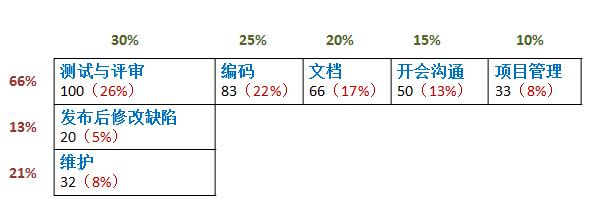
\includegraphics[width=10cm]{AR1成本占比.jpg}

测试与评审一般占开发工作量的30\%

测试与评审一般占总质量成本(包括发布后维护与改缺陷工作)的66\%

把所有工作量都加起来,测试与评审还是占最大(26\%) , 编码第二 (22\%)

\framebox{%
\begin{minipage}[t]{0.97\columnwidth}\raggedright
注意:`测试与评审`包括所有与缺陷相关的成本,包括单元测试、静态扫描、
评审与相关的缺陷修正, 而编码只包括设计与编写代码部分。
例如,有些人会觉得比例应该是:\\
开发30\%,测试和bug修改25\%,需求和设计20\%,项目管理和沟通20\%,文档5\%

但如果按上面的定义,开发部分很可能已包括单元测试、静态扫描与改正缺陷工作,
如把这些都归到测试评审里会变回类似上图的比例。\strut
\end{minipage}}

\hypertarget{reference}{%
\section{Reference}\label{reference}}

1. Jones, Capers: "Software Quality Metrics: Three Harmful Metrics and
Two Helpful Metrics" 2012.\\


